%%%%%%%%%%%%%%%%%%%%%%%%%%%%%%%%%%%%%%%%%%%%%%%%%%%%
% LECTURE 14
%%%%%%%%%%%%%%%%%%%%%%%%%%%%%%%%%%%%%%%%%%%%%%%%%%%%
\section*{Review of Nusselt Number}
\addcontentsline{toc}{section}{Review of Nusselt Number}
%%%%%%%%%%%%%%%%%%%%%%%%%%%%%%%%%%%%%%%%%%%%%%%%%%%%%%%%%%%%
The Nusselt number is a dimensionless parameter representing the solution at the boundary of the solid-liquid interface. It is defined as:

\[
    \left.\frac{\partial T^*}{\partial y^*}\right|_{y^*=0} = \text{Nu}_x = \frac{h \cdot x}{k_f} = f(x^*,\operatorname{Re_L},\operatorname{Pr}) = \frac{\text{conv. HT}}{\text{cond. HT}}
\]
%
also
\[
        \overline{\operatorname{Nu}} =\frac{\overline{h} \cdot L}{k_f} = f(\operatorname{Re_L}, \operatorname{Pr})
\]
%
If we know $\operatorname{Nu}$ then we can find $ h = \operatorname{Nu} \cdot k_f / L$. Nu is tabulated for different flows (table 7.7 and 8.4)
%
Similarly 
\[
           \text{friction coefficient: } C_f = \frac{2}{\operatorname{Re_L}} f(x^*,\operatorname{Re_L}) = \frac{2}{\operatorname{Re_L}}\frac{\partial u^*}{\partial y^*} \Bigl \vert_{y^*=0}
\]
%
It's important to note that:
%
\begin{itemize}
    \item A larger Nusselt number does not necessarily mean higher heat transfer (for the same problem)
    \item The average Nusselt number is not the average of local Nusselt numbers (it's defined using the average heat transfer coefficient)
\end{itemize}
%
\begin{definition}
In general
    \[
        \operatorname{Nu}_{x}=C \,\operatorname{Re}^m \cdot\operatorname{Pr}^n
    \]
    For turbulet, $m=0.8$ but for laminar $m=0.5$. Also for small Pr, we have $n=0.5$ but for Pr $\sim 1-1000$, we have $n = 1/3$.
\end{definition}

%%%%%%%%%%%%%%%%%%%%%%%%%%%%%%%%%%%%%%%%%%%%%%%%%%%%%%%%%%%%
\section*{Integral Method for Boundary Layer Problems}
\addcontentsline{toc}{section}{Integral Method for Boundary Layer Problems}
%%%%%%%%%%%%%%%%%%%%%%%%%%%%%%%%%%%%%%%%%%%%%%%%%%%%%%%%%%%%
The integral method provides an alternative approach to solve boundary layer problems:

\begin{itemize}
    \item Instead of solving differential equations directly, we apply conservation laws to a control volume
    \item We approximate the velocity and temperature profiles using polynomials
    \item This approach provides good physical insight and often produces remarkably accurate results at the interface
    \item The method is particularly valuable when exact solutions are unavailable
\end{itemize}
% %%%%%%%%%%%%%%%%%%%%%%%%%%%%%%%%%%%%%%%%%%%%%%%%%%%%%%%%%%%%
% \subsection*{Integral Analysis of Momentum Boundary Layer}
% \addcontentsline{toc}{subsection}{Integral Analysis of Momentum Boundary Layer}
% %%%%%%%%%%%%%%%%%%%%%%%%%%%%%%%%%%%%%%%%%%%%%%%%%%%%%%%%%%%%
% Consider a control volume within the boundary layer with height $h \geq \delta$ (where $\delta$ is the boundary layer thickness):

% \begin{figure}[h]
% % Placeholder for control volume figure
% \end{figure}

% \subsubsection*{Conservation of Mass}
% \addcontentsline{toc}{subsubsection}{Conservation of Mass}

% For the control volume, mass must be conserved. At the upstream face (1):
% \[
%     \dot{m}_1 = \int_0^h \rho u \, dy
% \]

% At the downstream face (2):
% \[
%     \dot{m}_2 = \int_0^h \rho u \, dy + \frac{d}{dx}\left(\int_0^h \rho u \, dy\right)dx
% \]

% For mass to be conserved, some fluid must leave through the top surface (a):
% \[
%     \dot{m}_a = \frac{d}{dx}\left(\int_0^h \rho u \, dy\right)dx
% \]
% %%%%%%%%%%%%%%%%%%%%%%%%%%%%%%%%%%%%%%%%%%%%%%%%%%%%%%%%%%%%
% \subsubsection*{Conservation of Momentum}
% \addcontentsline{toc}{subsubsection}{Conservation of Momentum}
% %%%%%%%%%%%%%%%%%%%%%%%%%%%%%%%%%%%%%%%%%%%%%%%%%%%%%%%%%%%%
% Momentum entering at face (1):
% \[
% \dot{M}_1 = \int_0^h \rho u^2 \, dy
% \]

% Momentum leaving at face (2):
% \[
% \dot{M}_2 = \int_0^h \rho u^2 \, dy + \frac{d}{dx}\left(\int_0^h \rho u^2 \, dy\right)dx
% \]

% Momentum leaving through the top surface:
% \[
%     \dot{M}_a = U_\infty \frac{d}{dx}\left(\int_0^h \rho u \, dy\right)dx
% \]

% Note that the fluid leaving the top of the control volume carries momentum with velocity $U_\infty$. The net change in momentum must equal the forces acting on the control volume. The only significant force is the wall shear stress $\tau_w$ (since the pressure gradient is zero for a flat plate):

% \[
%     \tau_w dx = -\frac{d}{dx}\left(\int_0^{\delta} \rho u(U_\infty - u) \, dy\right)dx
% \]

% where we use the fact that $(U_\infty - u) = 0$ for $y > \delta$.

% From the constitutive law for a Newtonian fluid:

% \[
%     \tau_w = \mu\left.\frac{\partial u}{\partial y}\right|_{y=0}
% \]

% Therefore:

% \[
% \mu\left.\frac{\partial u}{\partial y}\right|_{y=0} = -\frac{d}{dx}\left(\int_0^{\delta} \rho u(U_\infty - u) \, dy\right)
% \]
% %%%%%%%%%%%%%%%%%%%%%%%%%%%%%%%%%%%%%%%%%%%%%%%%%%%%%%%%%%%%
% \subsection*{Integral Analysis of Momentum Boundary Layer}
% \addcontentsline{toc}{subsection}{Integral Analysis of Momentum Boundary Layer}
% %%%%%%%%%%%%%%%%%%%%%%%%%%%%%%%%%%%%%%%%%%%%%%%%%%%%%%%%%%%%

% The Kármán momentum integral equation (KMIE) is a fundamental tool in boundary layer theory that allows for approximate solutions without solving the full Navier-Stokes equations. Developed by Theodore von Kármán in 1921, it applies conservation principles to the boundary layer as a whole rather than at each point. The equation takes the form:
% \[
%     \frac{d\theta}{dx} + \frac{\theta}{U_e}\frac{dU_e}{dx}(2+H) = \frac{\tau_w}{\rho U_e^2}
% \]
% %
% Where:
% \begin{itemize}
%     \item $\theta$ is the momentum thickness
%     \item $U_e$ is the velocity at the edge of the boundary layer (equivalent to $U_\infty$ for a flat plate)
%     \item $H = \delta^*/\theta$ is the shape factor, with $\delta^*$ being the displacement thickness
%     \item $\tau_w$ is the wall shear stress
%     \item $\rho$ is the fluid density
% \end{itemize}

% For the special case of a flat plate with zero pressure gradient ($\frac{dU_e}{dx} = 0$), the equation simplifies to:
% \[
%     \frac{d\theta}{dx} = \frac{\tau_w}{\rho U_\infty^2}
% \]

% This simplified form will be derived from first principles below.

%%%%%%%%%%%%%%%%%%%%%%%%%%%%%%%%%%%%%%%%%%%%%%%%%%%%%%%%%%%%
\subsection*{Derivation Using Control Volume Analysis}
\addcontentsline{toc}{subsection}{Derivation Using Control Volume Analysis}
%%%%%%%%%%%%%%%%%%%%%%%%%%%%%%%%%%%%%%%%%%%%%%%%%%%%%%%%%%%%

Consider a steady, incompressible, two-dimensional flow over a flat plate. We define a control volume that extends in the streamwise direction from $x$ to $x+dx$ and vertically from the wall ($y=0$) to a height $h$ where $h \geq \delta$ (the boundary layer thickness). For $y>\delta$ the velocity is constant at $U_\infty$.

\begin{figure}[H]
    \centering
    % Insert your control volume figure here.
    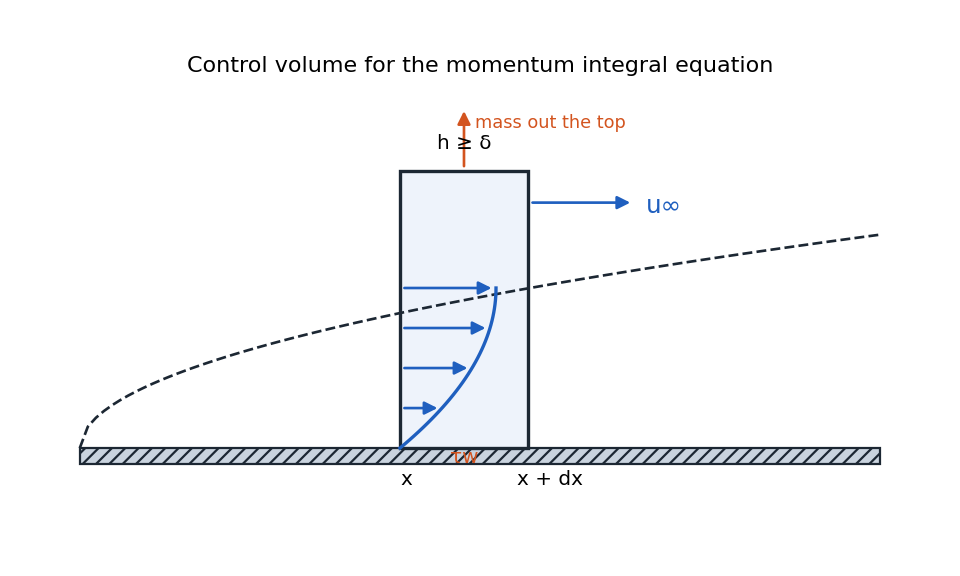
\includegraphics[width=0.5\linewidth]{pics/integral_method.png}
    \caption{Control volume within the momentum boundary layer.}
\end{figure}

\paragraph{Conservation of Mass}
For steady, incompressible flow, the mass entering and leaving the control volume must be balanced. The mass flow rates are:

\begin{itemize}
    \item At upstream face (face 1): $\dot{m}_1 = \int_0^h \rho\,u(y,x)\,dy$
    
    \item At downstream face (face 2): 
    \[
    \dot{m}_2 = \int_0^h \rho\,u(y,x+dx)\,dy \approx \dot{m}_1 + \frac{d}{dx}\left(\int_0^h \rho\,u\,dy\right)dx
    \]
    
    \item Vertical mass flux through top surface: $\dot{m}_a = \rho\,v\big|_{y=h}\,dx$
\end{itemize}

Mass conservation requires:
\[
\dot{m}_2 = \dot{m}_1 + \dot{m}_a
\]

Therefore:
\[
\frac{d}{dx}\left(\int_0^h \rho\,u\,dy\right) = \rho\,v\big|_{y=h}
\]

For constant density, this relation determines the entrainment velocity at the top of the control volume.

\paragraph{Conservation of Momentum}
Next, we apply momentum conservation to the same control volume.

The momentum fluxes are:
\begin{itemize}
    \item Momentum entering at face 1: $\dot{M}_1 = \int_0^h \rho\,u^2\,dy$
    
    \item Momentum leaving at face 2: 
    \[
    \dot{M}_2 = \int_0^h \rho\,u^2\,dy + \frac{d}{dx}\left(\int_0^h \rho\,u^2\,dy\right)dx
    \]
    
    \item Momentum carried by fluid exiting through top surface:
    \[
    \dot{M}_a = U_\infty\,\dot{m}_a = U_\infty\,\rho\,v\big|_{y=h}\,dx = U_\infty\,\frac{d}{dx}\left(\int_0^h \rho\,u\,dy\right)dx
    \]
\end{itemize}

\paragraph{Momentum Balance}
The net change in momentum must equal the force acting on the fluid. \textbf{For a flat plate with zero pressure gradient}, the only significant force is the wall shear stress $\tau_w$ acting over the wetted surface area $dx$:
\[
\tau_w\,dx = \dot{M}_1 - (\dot{M}_2 - \dot{M}_a)
\]

Substituting the expressions for $\dot{M}_1$, $\dot{M}_2$, and $\dot{M}_a$:
\[
    \begin{aligned}
    & -\tau_w d x=\frac{d}{d x}\left(\int_0^\delta \rho u^2 d y\right) d x-U_\infty \frac{d}{d x}\left(\int_0^\delta \rho u d y\right) d x 
    \\[0.5em]
    & -\tau_w=\frac{d}{d x}\left(\int_0^\delta \rho u^2 d y\right)-U_\infty \frac{d}{d x}\left(\int_0^\delta \rho u d y\right)
    \\[0.5em]
    & -\tau_w=\frac{d}{d x}\left(\int_0^\delta \rho u^2 d y\right)-\frac{d}{d x} \int_0^\delta \rho u U_\infty d y
    \\[0.5em]
    & \tau_w=\frac{d}{d x}\left[\int_0^\delta \rho u(U_\infty-u) d y\right]
    \\[0.5em]
    & \tau_w =\frac{d}{d x}\left[\rho U_\infty^2 \underbrace{\int_0^\delta \rho \frac{u}{U_\infty}\left(1-\frac{u}{U_\infty}\right) d y}_{\delta_M}\right]
    \end{aligned}
\]
%
Thus,
\[
    \frac{\tau_w}{\rho}=\frac{d}{d x}\left(U_\infty^2 \delta_M\right)
\]
\begin{definition}[KMIE]
Kármán Momentum Integral Equation (KMIE) for a flat plate defined as follows:
\[
    \frac{\tau_w}{\rho}=\frac{d}{d x}\left(U_\infty^2 \delta_M\right)
\]

%
where the momentum thickness $\delta_M$ is defined as:
\[
    \delta_M = \int_0^{\delta} \frac{u}{U_\infty}\left(1-\frac{u}{U_\infty}\right)dy
\]

\end{definition}

%
\textit{Note:} we assumed the pressure to be constant, so $dp/dx = dU_\infty/x = 0$.
%
This represents the loss of momentum flux in the boundary layer due to viscous effects. 
%
\paragraph{Alternative Form Using Wall Shear Stress}
For a Newtonian fluid, the wall shear stress is:
\[
    \tau_w = \mu\left.\frac{\partial u}{\partial y}\right|_{y=0}
\]

Therefore, the von Kármán momentum integral equation can also be written as:
\[
    \mu\left.\frac{\partial u}{\partial y}\right|_{y=0} = \rho U_\infty^2 \frac{d\delta_M}{dx} = \rho \frac{d}{d x} \int_0^\delta u\left(U_{\infty}-u\right)\;dy
\]


This form explicitly connects the local velocity gradient at the wall to the rate of change of momentum thickness along the plate.
%%%%%%%%%%%%%%%%%%%%%%%%%%%%%%%%%%%%%%%%%%%%%%%%%%%%%%%%%%%%%
\subsubsection*{Typical Methodology using KMIE}
\addcontentsline{toc}{subsubsection}{Typical Methodology using KMIE}{Typical Methodology using KMIE}
% %%%%%%%%%%%%%%%%%%%%%%%%%%%%%%%%%%%%%%%%%%%%%%%%%%%%%%%%%%%%
The typical methodology for using the KMIE is as follows:
\begin{enumerate}[(a)]
    \item Obtain an approximate expression for $U_\infty=U_\infty(x)$ from inviscid flow theory, e.g., potential flow theory. Recall that Bernoulli's equation can be used to relate the pressure and $U_\infty$.
    %
    \item Assume a velocity profile in the boundary layer subject to the appropriate boundary conditions, i.e., assume a form for,
    %
    $$
    \frac{u}{U_\infty}=f\left(\frac{y}{\delta}\right)
    $$
    %
    subject to the boundary conditions,
    %
    $$
    \frac{u}{U_\infty}\left(\frac{y}{\delta}=0\right)=0 \quad \text { and } \quad \frac{u}{U_\infty}\left(\frac{y}{\delta}=1\right)=1
    $$
    %
    The form of the approximate velocity profile is typically found based on curve fits to experimental measurements of the boundary layer velocity profile. Higher order profiles will have additional boundary conditions. For example, a cubic curve fit will also have a boundary condition that matches the slope of the velocity profile at the free stream boundary.
    %
    \item The shear stress at the wall for a laminar flow can also be determined from the Newtonian stress-strain rate constitutive relations to be,
    %
    $$
    \tau_w=\left.\mu\left(\frac{U_\infty}{\delta}\right) \frac{d(u / U_\infty)}{d(y / \delta)}\right|_{\frac{y}{\delta}=0}
    $$
    %
\end{enumerate}
%
% %%%%%%%%%%%%%%%%%%%%%%%%%%%%%%%%%%%%%%%%%%%%%%%%%%%%%%%%%%%%
% \subsubsection*{Velocity Profile Approximation}
% \addcontentsline{toc}{subsubsection}{Velocity Profile Approximation}
% %%%%%%%%%%%%%%%%%%%%%%%%%%%%%%%%%%%%%%%%%%%%%%%%%%%%%%%%%%%%

% To solve the integral equation, we approximate the velocity profile within the boundary layer using a third-order polynomial:

% \[
% \frac{u}{U_\infty} = a_0 + a_1\frac{y}{\delta} + a_2\left(\frac{y}{\delta}\right)^2 + a_3\left(\frac{y}{\delta}\right)^3
% \]

% The boundary conditions are:
% \begin{enumerate}
%     \item $u = 0$ at $y = 0$ (no-slip condition)
%     \item $u = U_\infty$ at $y = \delta$ (edge of boundary layer)
%     \item $\frac{\partial u}{\partial y} = 0$ at $y = \delta$ (smooth transition)
%     \item $\frac{\partial^2 u}{\partial y^2} = 0$ at $y = \delta$ (smooth transition)
% \end{enumerate}

% Applying these conditions yields:

% \[
% \frac{u}{U_\infty} = \frac{3}{2}\left(\frac{y}{\delta}\right) - \frac{1}{2}\left(\frac{y}{\delta}\right)^3
% \]

% Substituting this profile into the momentum integral equation and solving the resulting differential equation:

% \[
% \delta = 4.64\sqrt{\frac{\nu x}{U_\infty}}
% \]

% Or in dimensionless form:

% \[
% \frac{\delta}{x} = \frac{4.64}{\sqrt{\text{Re}_x}}
% \]

% The exact solution from the similarity method gives $\frac{\delta}{x} = \frac{5.0}{\sqrt{\text{Re}_x}}$, showing that the integral method is remarkably accurate (within ~7%).

% For the skin friction coefficient:

% \[
% C_f = \frac{\tau_w}{\frac{1}{2}\rho U_\infty^2} = \frac{0.646}{\sqrt{\text{Re}_x}}
% \]

% Compared to the exact value of $\frac{0.664}{\sqrt{\text{Re}_x}}$ (within ~3\%).

%%%%%%%%%%%%%%%%%%%%%%%%%%%%%%%%%%%%%%%%%%%%%%%%%%%%%%%%%%%%
\subsubsection*{Velocity Profile Approximation}
\addcontentsline{toc}{subsubsection}{Velocity Profile Approximation}
%%%%%%%%%%%%%%%%%%%%%%%%%%%%%%%%%%%%%%%%%%%%%%%%%%%%%%%%%%%%

To solve the momentum integral equation, we approximate the velocity profile within the boundary layer using a third-order polynomial:

\[
\frac{u}{U_\infty} = a_0 + a_1\frac{y}{\delta} + a_2\left(\frac{y}{\delta}\right)^2 + a_3\left(\frac{y}{\delta}\right)^3
\]
%
The boundary conditions are:
%
\begin{enumerate}
    \item \textbf{No-slip at the wall:} $u = 0$ at $y = 0$
    %
    \item \textbf{Matching the free stream:} $u = U_\infty$ at $y = \delta$
    %
    \item \textbf{Zero velocity gradient at the edge:} $\frac{\partial u}{\partial y} = 0$ at $y = \delta$
    %
    \item \textbf{Zero curvature at the edge:} $\frac{\partial^2 u}{\partial y^2} = 0$ at $y = \delta$
\end{enumerate}

Solving for the Coefficients, 
%
\[
    \boxed{
    \frac{u}{U_\infty} = \frac{3}{2}\left(\frac{y}{\delta}\right) - \frac{1}{2}\left(\frac{y}{\delta}\right)^3
    }
\]


%%%%%%%%%%%%%%%%%%%%%%%%%%%%%%%%%%%%%%%%%%%%%%%%%%%%%%%%%%%%
\subsubsection*{Momentum Integral Analysis}
\addcontentsline{toc}{subsubsection}{Momentum Integral Analysis}
%%%%%%%%%%%%%%%%%%%%%%%%%%%%%%%%%%%%%%%%%%%%%%%%%%%%%%%%%%%%

The momentum thickness $\delta_M$ is:
\[
    \delta_M = \int_0^\delta \frac{u}{U_\infty}\left(1-\frac{u}{U_\infty}\right)dy = \frac{39}{280}\delta 
\]
%
Using KMIE:
\[
    \frac{d}{d x}\left(\frac{39}{280} \rho U_{\infty}^2 \delta\right)= \left.\mu \frac{\partial u}{\partial y}\right|_{y=0}
\]
%
using our approximate solution for $u/U_\infty$:
\[
    \left.\mu \frac{\partial u}{\partial y}\right|_{y=0} = \frac{3}{2} \mu \frac{U_{\infty}}{\delta}
\]
%
Therefore,
\[
    \begin{aligned}
        & \frac{d}{d x}\left(\frac{39}{280} \rho U_{\infty}^2 \delta\right) = \frac{3}{2} \mu \frac{U_{\infty}}{\delta}
        \\[.5em]
        &\delta \cdot d \delta  =\frac{140}{13} \frac{\mu}{\rho U_\infty} d x
        \\[0.5em]
        &\frac{\delta^2}{2} =\frac{140}{13} \frac{\nu \cdot x}{U_\infty}+ \cancelto{0}{const.}
        \\[0.5em]
        & \boxed{
        \delta  =4.64 \sqrt{\frac{\nu x}{U_{\infty}}}
        } 
    \end{aligned}
\]
%
In dimensionless form, using the Reynolds number $\text{Re}_x = \frac{U_\infty x}{\nu}$:
%
\[
    \boxed{
        \frac{\delta}{x} = \frac{4.64}{\sqrt{\text{Re}_x}}
        }
\]

This compares well with the exact solution from the similarity method, which gives:
\[
\frac{\delta}{x} = \frac{5.0}{\sqrt{\text{Re}_x}}
\]

showing that the integral method is remarkably accurate (within ~7\%).

\paragraph{Skin Friction Coefficient}
Substituting $\tau_w$ and $\delta$ into local skin friction coefficient:
\[
    C_f = \frac{\tau_w}{\frac{1}{2}\rho U_\infty^2}  = \frac{0.646}{\sqrt{\text{Re}_x}}
\]
%
This compares well with the exact Blasius solution:
\[
    C_f = \frac{0.664}{\sqrt{\text{Re}_x}}
\]

demonstrating that our approximation is within ~3\% of the exact value.

% %%%%%%%%%%%%%%%%%%%%%%%%%%%%%%%%%%%%%%%%%%%%%%%%%%%%%%%%%%%%
% \subsection*{Integral Analysis of Thermal Boundary Layer}
% \addcontentsline{toc}{subsection}{Integral Analysis of Thermal Boundary Layer}
% %%%%%%%%%%%%%%%%%%%%%%%%%%%%%%%%%%%%%%%%%%%%%%%%%%%%%%%%%%%%

% We now apply a similar approach to the thermal boundary layer. For the case where $\delta_t < \delta$ (thermal boundary layer thinner than momentum boundary layer):
% %%%%%%%%%%%%%%%%%%%%%%%%%%%%%%%%%%%%%%%%%%%%%%%%%%%%%%%%%%%
% \subsubsection*{Energy Conservation}
% \addcontentsline{toc}{subsubsection}{Energy Conservation}
% %%%%%%%%%%%%%%%%%%%%%%%%%%%%%%%%%%%%%%%%%%%%%%%%%%%%%%%%%%%
% The energy equation for the control volume is:

% \[
% \rho c_p \frac{d}{dx}\left(\int_0^{\delta_t} u(T-T_\infty) \, dy\right) = -k\left.\frac{\partial T}{\partial y}\right|_{y=0}
% \]

% We assume that conduction in the x-direction is negligible compared to convection.
% %%%%%%%%%%%%%%%%%%%%%%%%%%%%%%%%%%%%%%%%%%%%%%%%%%%%%%%%%%%
% \subsubsection*{Temperature Profile Approximation}
% \addcontentsline{toc}{subsubsection}{Temperature Profile Approximation}
% %%%%%%%%%%%%%%%%%%%%%%%%%%%%%%%%%%%%%%%%%%%%%%%%%%%%%%%%%%%
% Similar to the velocity profile, we approximate the temperature profile with a third-order polynomial:

% \[
% \frac{T-T_\infty}{T_s-T_\infty} = a_0 + a_1\frac{y}{\delta_t} + a_2\left(\frac{y}{\delta_t}\right)^2 + a_3\left(\frac{y}{\delta_t}\right)^3
% \]

% Applying boundary conditions:
% \begin{enumerate}
%     \item $T = T_s$ at $y = 0$ (surface temperature)
%     \item $T = T_\infty$ at $y = \delta_t$ (edge of thermal boundary layer)
%     \item $\frac{\partial T}{\partial y} = 0$ at $y = \delta_t$ (smooth transition)
%     \item $\frac{\partial^2 T}{\partial y^2} = 0$ at $y = 0$ (from energy equation at the wall)
% \end{enumerate}

% Solving for the coefficients:

% \[
% \frac{T-T_\infty}{T_s-T_\infty} = 1 - \frac{3}{2}\left(\frac{y}{\delta_t}\right) + \frac{1}{2}\left(\frac{y}{\delta_t}\right)^3
% \]

% Substituting this profile and the velocity profile into the energy integral equation:

% \[
% \frac{\delta_t}{\delta} = \zeta = C\left(\frac{x}{x-x_0}\right)^{3/4}\text{Pr}^{-1/3}
% \]

% Where $x_0$ is the point where heating begins (which may be different from the leading edge).
% %%%%%%%%%%%%%%%%%%%%%%%%%%%%%%%%%%%%%%%%%%%%%%%%%%%%%%%%%%%
% \subsubsection*{Heat Transfer Coefficient and Nusselt Number}
% \addcontentsline{toc}{subsubsection}{Heat Transfer Coefficient and Nusselt Number}
% %%%%%%%%%%%%%%%%%%%%%%%%%%%%%%%%%%%%%%%%%%%%%%%%%%%%%%%%%%%
% The heat transfer coefficient is:

% \[
% h = \frac{-k\left.\frac{\partial T}{\partial y}\right|_{y=0}}{T_s-T_\infty} = \frac{3k}{2\delta_t}
% \]

% For the case where heating begins at the leading edge ($x_0 = 0$):

% \[
% \text{Nu}_x = \frac{hx}{k} = 0.332 \, \text{Re}_x^{1/2} \, \text{Pr}^{1/3}
% \]

% This exactly matches the result obtained from the similarity solution, which is remarkably fortunate given the approximations made.

% For the case where heating begins at some point $x_0 > 0$:

% \[
% \text{Nu}_x = 0.332 \, \text{Re}_x^{1/2} \, \text{Pr}^{1/3} \left(1-\left(\frac{x_0}{x}\right)^{3/4}\right)^{-1/3} \, H(x-x_0)
% \]

% Where $H(x-x_0)$ is the Heaviside step function that equals 0 for $x < x_0$ and 1 for $x \geq x_0$.

% %%%%%%%%%%%%%%%%%%%%%%%%%%%%%%%%%%%%%%%%%%%%%%%%%%%%%%%%%%%%
% \subsection*{Integral Analysis of Thermal Boundary Layer}
% \addcontentsline{toc}{subsection}{Integral Analysis of Thermal Boundary Layer}
% %%%%%%%%%%%%%%%%%%%%%%%%%%%%%%%%%%%%%%%%%%%%%%%%%%%%%%%%%%%%

% Just as we analyzed the momentum boundary layer using integral methods, we can apply a similar approach to the thermal boundary layer that develops when a fluid flows over a heated (or cooled) surface. The thermal boundary layer represents the region where temperature gradients exist in the fluid.

% \paragraph{Thermal Boundary Layer Thickness}
% The thermal boundary layer thickness $\delta_t$ is defined as the distance from the wall where:
% \[
% \frac{T - T_\infty}{T_s - T_\infty} = 0.99
% \]

% Where $T_s$ is the surface temperature and $T_\infty$ is the free stream temperature. In general, the thermal boundary layer thickness $\delta_t$ differs from the momentum boundary layer thickness $\delta$. The ratio $\delta_t/\delta$ depends on the Prandtl number (Pr) of the fluid, which relates momentum diffusivity to thermal diffusivity.

% We now focus on the case where $\delta_t < \delta$ (thermal boundary layer thinner than momentum boundary layer), which is typically the case for fluids with Pr > 1, such as water and oils.

% %%%%%%%%%%%%%%%%%%%%%%%%%%%%%%%%%%%%%%%%%%%%%%%%%%%%%%%%%%%
% \subsubsection*{Energy Conservation}
% \addcontentsline{toc}{subsubsection}{Energy Conservation}
% %%%%%%%%%%%%%%%%%%%%%%%%%%%%%%%%%%%%%%%%%%%%%%%%%%%%%%%%%%%

% Similar to how we derived the momentum integral equation, we can apply conservation of energy to a control volume within the thermal boundary layer. The energy balance considers:

% \begin{itemize}
%     \item Energy advected into and out of the control volume by fluid flow
%     \item Energy transferred by conduction at the wall
% \end{itemize}

% The resulting thermal energy integral equation is:
% \[
% \rho c_p \frac{d}{dx}\left(\int_0^{\delta_t} u(T-T_\infty) \, dy\right) = -k\left.\frac{\partial T}{\partial y}\right|_{y=0}
% \]

% Where:
% \begin{itemize}
%     \item $\rho$ is the fluid density
%     \item $c_p$ is the specific heat at constant pressure
%     \item $u$ is the velocity component in the x-direction
%     \item $T$ is the temperature
%     \item $k$ is the thermal conductivity
%     \item $\left.\frac{\partial T}{\partial y}\right|_{y=0}$ represents the temperature gradient at the wall
% \end{itemize}

% The left side of the equation represents the streamwise rate of change of thermal energy deficit within the boundary layer, while the right side represents the heat flux from the wall into the fluid.

% We assume that conduction in the x-direction is negligible compared to convection, which is valid for high Reynolds number flows. This simplification aligns with boundary layer theory assumptions.

% %%%%%%%%%%%%%%%%%%%%%%%%%%%%%%%%%%%%%%%%%%%%%%%%%%%%%%%%%%%
% \subsubsection*{Temperature Profile Approximation}
% \addcontentsline{toc}{subsubsection}{Temperature Profile Approximation}
% %%%%%%%%%%%%%%%%%%%%%%%%%%%%%%%%%%%%%%%%%%%%%%%%%%%%%%%%%%%

% To solve the thermal integral equation, we need to specify the temperature distribution within the thermal boundary layer. Following our approach for the velocity profile, we approximate the temperature profile with a third-order polynomial:
% \[
% \frac{T-T_\infty}{T_s-T_\infty} = a_0 + a_1\frac{y}{\delta_t} + a_2\left(\frac{y}{\delta_t}\right)^2 + a_3\left(\frac{y}{\delta_t}\right)^3
% \]

% The coefficients are determined by applying appropriate boundary conditions. These conditions ensure physical realism and continuity at the boundaries:

% \begin{enumerate}
%     \item $T = T_s$ at $y = 0$ (surface temperature)
    
%     This condition means that the fluid temperature at the wall equals the wall temperature, reflecting the no-slip condition and perfect thermal contact.
    
%     \item $T = T_\infty$ at $y = \delta_t$ (edge of thermal boundary layer)
    
%     By definition, at the edge of the thermal boundary layer, the fluid temperature approaches the free stream temperature.
    
%     \item $\frac{\partial T}{\partial y} = 0$ at $y = \delta_t$ (smooth transition)
    
%     This ensures a smooth transition between the boundary layer and the free stream, avoiding non-physical discontinuities in the temperature gradient.
    
%     \item $\frac{\partial^2 T}{\partial y^2} = 0$ at $y = 0$ (from energy equation at the wall)
    
%     This condition derives from the energy equation at the wall. For a flat plate with zero pressure gradient and constant wall temperature, the second derivative of temperature vanishes at the wall.
% \end{enumerate}

% Applying these boundary conditions to our polynomial and solving the resulting system of equations for the coefficients $a_0, a_1, a_2, a_3$:

% Condition 1 gives:
% \[
% 1 = a_0 \quad \Rightarrow \quad a_0 = 1
% \]

% Condition 2 gives:
% \[
% 0 = 1 + a_1 + a_2 + a_3 \quad \Rightarrow \quad a_1 + a_2 + a_3 = -1
% \]

% Condition 3 yields:
% \[
% \left.\frac{\partial}{\partial y}\left(\frac{T-T_\infty}{T_s-T_\infty}\right)\right|_{y=\delta_t} = \frac{a_1}{\delta_t} + \frac{2a_2}{\delta_t}\frac{\delta_t}{\delta_t} + \frac{3a_3}{\delta_t}\left(\frac{\delta_t}{\delta_t}\right)^2 = 0
% \]
% \[
% \Rightarrow a_1 + 2a_2 + 3a_3 = 0
% \]

% From condition 4:
% \[
% \left.\frac{\partial^2}{\partial y^2}\left(\frac{T-T_\infty}{T_s-T_\infty}\right)\right|_{y=0} = \frac{2a_2}{\delta_t^2} + \frac{6a_3}{\delta_t^2} \cdot 0 = 0
% \]
% \[
% \Rightarrow a_2 = 0
% \]

% Solving this system:
% \[
% a_0 = 1, \quad a_2 = 0
% \]

% From $a_1 + 2a_2 + 3a_3 = 0$ and $a_2 = 0$:
% \[
% a_1 + 3a_3 = 0 \quad \Rightarrow \quad a_1 = -3a_3
% \]

% From $a_1 + a_2 + a_3 = -1$ and $a_2 = 0$:
% \[
% a_1 + a_3 = -1
% \]

% Substituting $a_1 = -3a_3$:
% \[
% -3a_3 + a_3 = -1 \quad \Rightarrow \quad -2a_3 = -1 \quad \Rightarrow \quad a_3 = \frac{1}{2}
% \]

% Therefore:
% \[
% a_1 = -3 \cdot \frac{1}{2} = -\frac{3}{2}
% \]

% The resulting temperature profile is:
% \[
% \frac{T-T_\infty}{T_s-T_\infty} = 1 - \frac{3}{2}\left(\frac{y}{\delta_t}\right) + \frac{1}{2}\left(\frac{y}{\delta_t}\right)^3
% \]

% \paragraph{Thermal Boundary Layer Growth}
% Substituting this temperature profile and the previously determined velocity profile into the energy integral equation allows us to derive a relationship for the thermal boundary layer thickness:
% \[
% \frac{\delta_t}{\delta} = \zeta = C\left(\frac{x}{x-x_0}\right)^{3/4}\text{Pr}^{-1/3}
% \]

% Where:
% \begin{itemize}
%     \item $C$ is a constant determined from the analysis
%     \item $x_0$ is the point where heating begins (which may be different from the leading edge)
%     \item Pr is the Prandtl number ($\text{Pr} = \frac{\nu}{\alpha} = \frac{\mu c_p}{k}$)
% \end{itemize}

% This relationship shows how the thermal boundary layer thickness relates to the momentum boundary layer thickness. For high Prandtl number fluids, the thermal boundary layer is thinner than the momentum boundary layer, as thermal diffusion is slower than momentum diffusion.

% %%%%%%%%%%%%%%%%%%%%%%%%%%%%%%%%%%%%%%%%%%%%%%%%%%%%%%%%%%%
% \subsubsection*{Heat Transfer Coefficient and Nusselt Number}
% \addcontentsline{toc}{subsubsection}{Heat Transfer Coefficient and Nusselt Number}
% %%%%%%%%%%%%%%%%%%%%%%%%%%%%%%%%%%%%%%%%%%%%%%%%%%%%%%%%%%%

% The local heat transfer coefficient $h$ is defined by:
% \[
% q_w = h(T_s - T_\infty)
% \]

% Where $q_w$ is the heat flux at the wall. From Fourier's law:
% \[
% q_w = -k\left.\frac{\partial T}{\partial y}\right|_{y=0}
% \]

% Using our temperature profile:
% \[
% \left.\frac{\partial T}{\partial y}\right|_{y=0} = (T_s - T_\infty)\left.\frac{\partial}{\partial y}\left(\frac{T-T_\infty}{T_s-T_\infty}\right)\right|_{y=0} = (T_s - T_\infty)\left.\frac{\partial}{\partial y}\left(1 - \frac{3}{2}\frac{y}{\delta_t} + \frac{1}{2}\left(\frac{y}{\delta_t}\right)^3\right)\right|_{y=0}
% \]

% \[
% = (T_s - T_\infty)\left(-\frac{3}{2}\frac{1}{\delta_t}\right) = -\frac{3(T_s - T_\infty)}{2\delta_t}
% \]

% Therefore:
% \[
% q_w = k\frac{3(T_s - T_\infty)}{2\delta_t}
% \]

% And the heat transfer coefficient is:
% \[
% h = \frac{q_w}{T_s-T_\infty} = \frac{3k}{2\delta_t}
% \]

% \paragraph{Nusselt Number Derivation}
% The Nusselt number, which represents the dimensionless heat transfer coefficient, is defined as:
% \[
% \text{Nu}_x = \frac{hx}{k}
% \]

% Substituting the expression for $h$ and the relationship for $\delta_t$:
% \[
% \text{Nu}_x = \frac{3k}{2\delta_t} \cdot \frac{x}{k} = \frac{3x}{2\delta_t}
% \]

% For the case where heating begins at the leading edge ($x_0 = 0$), and considering the relationship between $\delta_t$ and $\delta$, along with the expression for $\delta$ in terms of Reynolds number:
% \[
% \text{Nu}_x = 0.332 \, \text{Re}_x^{1/2} \, \text{Pr}^{1/3}
% \]

% This result exactly matches the one obtained from the similarity solution developed by Pohlhausen, which is remarkably fortunate given the approximations made in the integral approach. This agreement validates the integral method for thermal boundary layer analysis.

% \paragraph{Unheated Starting Length Correction}
% For the case where heating begins at some point $x_0 > 0$ (known as unheated starting length):
% \[
% \text{Nu}_x = 0.332 \, \text{Re}_x^{1/2} \, \text{Pr}^{1/3} \left(1-\left(\frac{x_0}{x}\right)^{3/4}\right)^{-1/3} \, H(x-x_0)
% \]

% Where $H(x-x_0)$ is the Heaviside step function that equals 0 for $x < x_0$ and 1 for $x \geq x_0$.

% The term $\left(1-\left(\frac{x_0}{x}\right)^{3/4}\right)^{-1/3}$ represents a correction factor that accounts for the thickness of the momentum boundary layer that has already developed before heating begins. As $x$ increases relative to $x_0$, this correction factor approaches 1, and the Nusselt number approaches the standard result for heating from the leading edge.


%%%%%%%%%%%%%%%%%%%%%%%%%%%%%%%%%%%%%%%%%%%%%%%%%%%%%%%%%%%%
\subsection*{Integral Analysis of Thermal Boundary Layer}
\addcontentsline{toc}{subsection}{Integral Analysis of Thermal Boundary Layer}
%%%%%%%%%%%%%%%%%%%%%%%%%%%%%%%%%%%%%%%%%%%%%%%%%%%%%%%%%%%%

\paragraph{Thermal Boundary Layer Thickness}
The thermal boundary layer thickness \(\delta_t\) is defined as the distance from the surface at which the temperature reaches approximately 99\% of the free stream temperature:
\[
    \frac{T - T_\infty}{T_s - T_\infty} = 0.99
\]
%
Two main scenarios exist: either the thermal boundary layer is thicker (\(\delta_t > \delta\)), typical for low Prandtl number fluids (e.g., liquid metals), or thinner (\(\delta_t < \delta\)), common for fluids like water and oils (\(\mathrm{Pr} > 1\)). Here, we focus on the second scenario, \(\delta > \delta_t\).
%
\begin{figure}[H]
\centering
\begin{tikzpicture}[>=stealth,scale=0.7]
    % Define convenient lengths for dx and dy (adjust as desired)
    \def\dx{4}
    \def\dy{4}

    % 1) Draw the control-volume rectangle
    \draw[thick,green!50!black] (0,0) rectangle (\dx,\dy);

    % 3) Conduction at the bottom edge
    \draw[<-] (\dx/2,0) -- ++(0,-2)
      node[midway,right]
      {$-\left.k d x \frac{d T}{d y}\right|_{y=0}$} ;

    % 4) Conduction at the top edge (Taylor expansion form)
    \draw[->] (\dx/2,\dy) -- ++(0,2)
      node[midway,right,align=left]
      {$-\rho c_p  \frac{d}{d x}\left[\int_0^H u \,T_{\infty} d y\right] d x$};

    % 5) Convection at the left edge
    \draw[<-] (0,\dy/2) -- ++(-2,0)
      node[left]
      {$\rho c_p \int_0^H u T d y$};

    % 6) Convection at the right edge
    \draw[->] (\dx,\dy/2) -- ++(2,0)
      node[right]
      {$\rho c_p\left[\int_0^H(u T d y)+\frac{d}{d x}\left(\int_0^H u T d y\right) d x\right]$};
\end{tikzpicture}
\caption{Schematic of the control volume showing conduction and convection terms.}
\end{figure}
\paragraph{Integral Energy Equation}
Applying energy conservation to a control volume within the thermal boundary layer, we have:
%
\[
    \begin{aligned}
        \cancel{\rho c_p \int_0^H u T \,dy} - k\left.\frac{\partial T}{\partial y}\right|_{y=0}dx = \rho c_p\left[\cancel{\int_0^H u T \,dy} + \frac{d}{dx}\left(\int_0^H u T \,dy\right)dx\right]
        \\[0.5em]
        - \rho c_p  \frac{d}{dx}\left(\int_0^H u\, T_\infty\,dy\right)dx        
    \end{aligned}
\]
%
For $y>\delta_t$, our integral become 0 since $T=T_\infty$. Rearranging, we obtain the simplified energy integral equation:
\begin{definition}[KMIE for temperature profile]
\[
    \frac{d}{dx}\left[\int_0^{\textcolor{red}{\delta_t}} (T_\infty - T) u \,dy\right] = \alpha \left.\frac{\partial T}{\partial y}\right|_{y=0}
\]
\end{definition}
%
\paragraph{Polynomial Temperature Profile Approximation}
We approximate the temperature distribution using a cubic polynomial:
\[
        \theta^* = \frac{\theta}{\theta_\infty} = \frac{T - T_s}{T_\infty - T_s} = C_1 + C_2 y + C_3 y^2 + C_4 y^3
\]

The boundary conditions are:
\[
    \begin{aligned}
    & y=0, \quad T=T_s \quad \Rightarrow \quad \theta^* = 0 \\
    & y=\delta_t, \quad T=T_\infty \quad \Rightarrow \quad \theta^* = 1 \\
    & \left.\frac{\partial^2 T}{\partial y^2}\right|_{y=0}=0 \\
    & \left.\frac{\partial T}{\partial y}\right|_{y=\delta_t}=0
    \end{aligned}
\]

Applying these conditions and solving for coefficients, we get the temperature profile as given in the professor’s notes:
\[
    \theta^* =  \frac{T - T_s}{T_\infty - T_s} = \frac{3}{2}\frac{y}{\delta_t} - \frac{1}{2}\left(\frac{y}{\delta_t}\right)^3
\]

\paragraph{Solving the Integral Equation}
Substituting the velocity profile \(u/U_\infty = \frac{3}{2} \frac{y}{\delta}-\frac{1}{2}\left(\frac{y}{\delta}\right)^3\) and temperature profile into the integral energy equation, and defining the thickness ratio \(\zeta = \delta_t/\delta\), leads to the differential equation (from class notes):
\[
    \frac{3}{20} U_\infty \theta_\infty\frac{d}{dx}(\delta \zeta^2) = \frac{3}{2}\alpha\frac{\theta_\infty}{\zeta \delta}
\]

After simplifications, we have the linear ODE:
\[
    \begin{aligned}
            & \zeta^3+ 4 x \zeta^2 \frac{d \zeta}{d x}=\frac{13}{14} \frac{\alpha}{\nu}
            \\[0.5em]
            &\zeta^3 + \frac{4}{3} x \frac{d \zeta^3}{dx} = \frac{13}{14}\frac{\alpha}{\nu}
    \end{aligned}
\]

Solving the ODE, we obtain:
\[
\zeta^3 = C x^{-3/4} + \frac{13}{14}\frac{\alpha}{\nu}
\]

Applying the boundary condition \(\zeta(x_0)=0\) at the starting heating point \(x=x_0\), gives:
\[
C = -\frac{13}{14}\frac{x_0^{3/4}}{\mathrm{Pr}}
\]
%
Thus, the final thickness ratio expression is:
\begin{definition}
\[
    \zeta = \frac{\delta_t}{\delta} = \frac{1}{1.026}\mathrm{Pr}^{-1/3}\left[1-\left(\frac{x_0}{x}\right)^{3/4}\right]^{1/3}
\]    
\end{definition}
%
\paragraph{Unheated source} If velocity boundary layer growth begins at $x=0$, while thermal boundary layer development begins at $x=x_0$ (in textbook instead of $x_0$ they used $\xi$ notation). Hence there is no heat transfer for $0 \leq x \leq x_0$:
%
\begin{figure}[H]
    \centering
    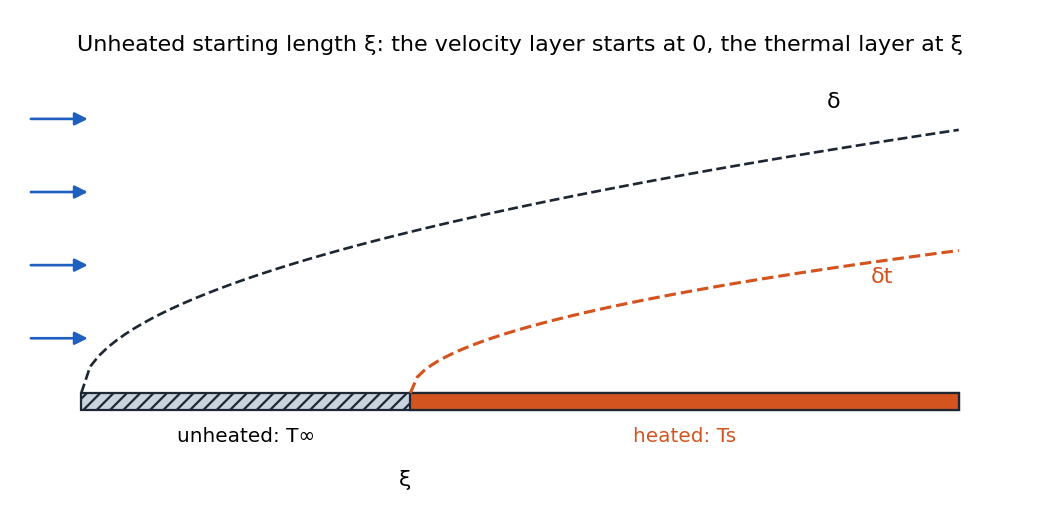
\includegraphics[width=0.65\linewidth]{pics/unheated_source.png}
    \caption{Flat plate in parallel flow with unheated starting length.}
\end{figure}
%
\begin{definition}
\[
    \zeta = \frac{\delta_t}{\delta} = \frac{1}{1.026}\mathrm{Pr}^{-1/3}\left[1-\left(\frac{x_0}{x}\right)^{3/4}\right]^{1/3}H(x - x_0)
\]
\end{definition}
%
where \(H(x - x_0)\) is the Heaviside function:
\[
H(x - x_0) = \begin{cases}
0 & x < x_0\\
1 & x \geq x_0
\end{cases}
\]
%
When heating begins at the leading edge (\(x_0=0\)), this simplifies to:
\begin{definition}
    \[
    \frac{\delta_t}{\delta} = \frac{1}{1.026}\mathrm{Pr}^{-1/3}
    \]
\end{definition}
%
\paragraph{Local Heat Transfer Coefficient and Nusselt Number}
The wall heat flux \(q''_s\) from Fourier’s law is:
\[
q''_s = -k\left.\frac{\partial T}{\partial y}\right|_{y=0} = \frac{3}{2}\frac{k(T_s - T_\infty)}{\delta_t}
\]
\begin{definition}
The local heat transfer coefficient is:
\[
    h_x = \frac{q''_s}{T_s - T_\infty} = \frac{3k}{2\delta_t}
\]

Substituting \(\delta_t\) into this expression, the local Nusselt number \(\mathrm{Nu}_x\) is:

\[
    \mathrm{Nu}_x = \frac{h_x x}{k} = 0.332 \mathrm{Pr}^{1/3}\mathrm{Re}_x^{1/2}\left[1-\left(\frac{x_0}{x}\right)^{3/4}\right]^{-1/3} \ \ (x>x_0)
\]
%
\[
    \mathrm{Nu}_x = 0.332\,\mathrm{Pr}^{1/3}\,\mathrm{Re}_x^{1/2}
\]
\end{definition}

%
\textit{Note 1:} For $h_x$ we can not use Heaviside function because if $x<x_0$ then $h_x$ is not defined not zero. But $\delta_t$ is zero so using Heaviside there is appropriate.
\\[0.5em]
\textit{Note 2:} This integral method result matches the exact solution.



%%%%%%%%%%%%%%%%%%%%%%%%%%%%%%%%%%%%%%%%%%%%%%%%%%%%%%%%%%%
% \subsection*{Applications of the Integral Method}
% \addcontentsline{toc}{subsection}{Applications of the Integral Method}
%%%%%%%%%%%%%%%%%%%%%%%%%%%%%%%%%%%%%%%%%%%%%%%%%%%%%%%%%%%
% The integral method is particularly valuable for:

% \begin{enumerate}
%     \item Problems with complex boundary conditions, such as spatially varying surface temperature
%     \item Unheated starting length problems where heating begins downstream of the leading edge
%     \item Problems where superposition principles can be applied
% \end{enumerate}

% For a spatially varying surface temperature $T_s(x)$, we can use the step function solution as a building block and apply superposition principles to construct the solution.
